\chapter{Evaluation}
\renewcommand{\baselinestretch}{\mystretch}
\label{chap:Eval}
%\setlength{\parindent}{0pt}

\section{Locale issue}

\cmt{Unable to build Vixen solution because of system locale, special character and file encoding issue. \wn{1}}

\section{Original performance}

\fref{fig:original} shows the performance of the original Vixen execution engine. The CPU usage frequently reaches above $90 \%$, while the refresh rate being very unstable around the configured 20 fps. Especially at the first 60 seconds, the refresh rate drops to 5 fps trying to keep up with element updates. \wn{2}

\begin{figure}[t]
    \centering
    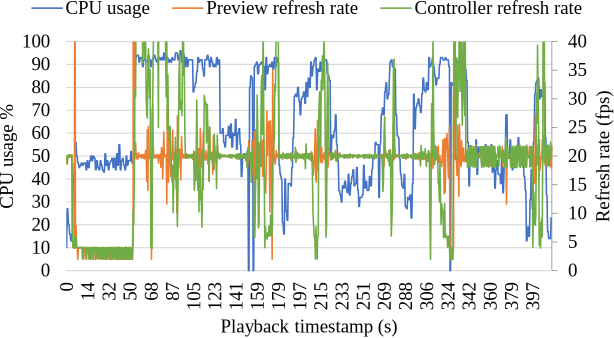
\includegraphics[width=0.8\columnwidth]{original}
    \caption{Performance of Vixen execution engine}
    \label{fig:original}
\end{figure}

Further analysis using Microsoft Visual Studio's sampling profiler shows, around $65 \%$ of CPU time was wasted between translation layers for generating controller commands, while the actual command assignment taking less than $1 \%$ of CPU time. There are several different command formats possible, for example 8-bit, 16-bit and RGB channels. Therefore, the application need to resolve the actual format of commands from their base type, which is apparently very inefficient in C\#. This process is called \texttt{dispatch} in the source code, it must be reduced or removed to improve performance. \wn{3}

The implementation of preview display was also inefficient, using around $20 \%$ CPU time in later stages.

\cmt{Different real-world sequence examples}

\section{Performance on Linux}

\cmt{Necessary GUI modification, imperfect GUI, tested with mono.}

\cmt{Insert screenshots...}

\section{Extract rendered sequence}

Instead of trying to improve the original execution engine, the performance problem may be eliminated by playing back stored data frames directly to individual hardware controllers. Thus, two steps are needed. Pre-rendering the sequence with accurate frame interval, then playback the rendered data to the controllers.

\section{Custom controller}

A custom controller module was developed based on one of its existing controllers. This controller uses TCP connection to transfer display data, supporting up to 65535 channels. A corresponding server application that simulates a multi-channel display was also developed using C++ and OpenGL \cite{shreiner2009opengl} rendering. Having this configuration allows debugging real-time display output without the need of a complex actual lighting controller setup. Data dumping, performance and statistical analysis can also be easily achieved. \wn{4}

The server application consumes less than $3 \%$ of CPU time under 50 fps refresh rate, which is negligible. It can also be executed on other computers, simulating real world network connection scenarios.

\section{Export sequence}

Although the custom controller module is capable of dumping outputs, it would not give the indication of sequence start and end information, and can have unstable frame rates influenced by CPU usage. Therefore, the sequence export function from sequence editor was used to dumping outputs.

The export function was originally used to convert the display sequence to formats recognisable by other applications and controllers. Most importantly, it renders the sequence using a manual timing source, gives accurate constant interval data dumps and controller channel mapping information. A customised data format was added to the export wizard, that can be later used for playback. \wn{5}

\cmt{Example XML file content?}

\cmt{Custom resolution modification?}

\cmt{Insert screenshots...}

